\documentclass[fleqn,10pt]{paper}

\usepackage[left=2cm,right=2cm,
top=0.5cm,
bottom=1.5cm,%
headheight=11pt,%
letterpaper]{geometry}



\usepackage[left=2cm,right=2cm,
			top=1.25cm,
			bottom=2.25cm,%
			headheight=11pt,%
			letterpaper]{geometry}
			
\frenchspacing			

\nonstopmode




\usepackage{lmodern}
\usepackage[T1]{fontenc}
\usepackage[utf8]{inputenc}



\usepackage{noweb}

\usepackage{multicol}
\usepackage{fancyhdr}
\usepackage{blindtext,graphicx}
\usepackage[absolute]{textpos}
%\usepackage[parfill]{parskip}
\usepackage{parskip}
\setlength{\parskip}{\baselineskip}

\usepackage[colorlinks=true,citecolor=brown]{hyperref}
\usepackage{gensymb}
\usepackage{csquotes}
\usepackage{amsmath}
\usepackage{fontawesome}
\usepackage{orcidlink}
\usepackage{standalone}
\usepackage{pdfpages}
\usepackage{subfiles}
\usepackage{svg}
\usepackage{sidecap}
\usepackage{float}
\usepackage{amssymb}
\usepackage{textcomp}
\usepackage{lettrine}
%\usepackage[T1]{fontenc}

\usepackage{soul}


%\usepackage{draftwatermark}
%\SetWatermarkText{DRAFT}
%\SetWatermarkScale{0.25}

\usepackage{booktabs,caption}
\usepackage[flushleft]{threeparttable}

%\usepackage{biblatex}
\usepackage[backend=bibtex8, sorting=none, style=chem-angew]{biblatex}

\let\cite\footfullcite

%\let\cite\footcite

\addbibresource{processed.bib}
%biblatex has a zoterordfxml
% might avoid the need for python bibtex_collections.py



\usepackage{etoolbox}
\AtBeginEnvironment{quote}{\small}




\usepackage{pifont}
\newcommand{\cmark}{\ding{51}}%
\newcommand{\xmark}{\ding{55}}%


\newcommand{\citationneeded}[1][]{\textsuperscript{[\color{blue}{\it \bf{citation needed}#1}]}}
\newcommand{\dubiousdiscuss}[1][]{\textsuperscript{\color{blue} [{\it \bf{dubious-discuss}}]} }

\newcommand{\light}[1]{\textcolor{gray}{#1}}

%
%
\usepackage{titlesec}
%
%% custom section


\titleformat{\section}
{\normalfont\LARGE\bfseries}{\thesection}{1em}{}
%\titleformat{\section}
%{\normalfont\LARGE\bfseries\PRLsep}
%{{{{\itshape \thesection\hskip 9pt\textpipe\hskip 9pt}}}}{0pt}{}
%
%% custom section
%\titleformat{\subsection}
%{\normalfont\Large\bfseries\PRLsep}
%{{{{\itshape \thesection\hskip 9pt\textpipe\hskip 9pt}}}}{0pt}{}
%
%
%


\newcommand{\Wsqm}{$\text{ W/m}^2$}

\newcommand{\ghfile}[1]{\href{https://github.com/0xDBFB7/covidinator/tree/master/#1}{\faGithub/\url{#1} }}

%\newcommand{\supercite}[1]{}
%\newcommand{\supercollect}[1]{}


\newlength{\PRLlen}
\newcommand*\PRLsep[1]{{\itshape \Large\settowidth{\PRLlen}{#1}\advance\PRLlen by -\textwidth\divide\PRLlen by -2\noindent\makebox[\the\PRLlen]{\resizebox{\the\PRLlen}{1pt}{$\blacktriangleleft$}}\raisebox{-.5ex}{#1}\makebox[\the\PRLlen]{\resizebox{\the\PRLlen}{1pt}{$\blacktriangleright$}}\bigskip}}


\renewcommand{\thefootnote}{\textcolor{gray}{\arabic{footnote}}}


\usepackage{graphicx}
\graphicspath{ {../media/} 
				{../firmware/eppenwolf/runs/sic_susceptor/} 
			}

\usepackage{tcolorbox}
\newtcolorbox{protocol}{colback=yellow!5!white,colframe=yellow!75!black}
\newtcolorbox{equipment}{colback=orange!5!white,colframe=orange!75!black}
\newtcolorbox{autem}{colback=red!5!white,colframe=red!75!black}
\newtcolorbox{toolchain}{colback=blue!5!white,colframe=blue!40!black!40}
\newtcolorbox{sidenote}{colback=cyan!5!white,colframe=blue!40!black!40}
%https://tex.stackexchange.com/questions/66154/how-to-construct-a-coloured-box-with-rounded-corners

%\usepackage[sfdefault,light]{roboto}

\setlength{\TPHorizModule}{1cm}
\setlength{\TPVertModule}{1cm}





%%%%********************************************************************
% fancy quotes
\definecolor{quotemark}{gray}{0.7}
\makeatletter
\def\fquote{%
	\@ifnextchar[{\fquote@i}{\fquote@i[]}%]
}%
\def\fquote@i[#1]{%
	\def\tempa{#1}%
	\@ifnextchar[{\fquote@ii}{\fquote@ii[]}%]
}%
\def\fquote@ii[#1]{%
	\def\tempb{#1}%
	\@ifnextchar[{\fquote@iii}{\fquote@iii[]}%]
}%
\def\fquote@iii[#1]{%
	\def\tempc{#1}%
	\vspace{1em}%
	\noindent%
	\begin{list}{}{%
			\setlength{\leftmargin}{0.1\textwidth}%
			\setlength{\rightmargin}{0.1\textwidth}%
		}%
		\item[]%
		\begin{picture}(0,0)%
		\put(-15,-5){\makebox(0,0){\scalebox{3}{\textcolor{quotemark}{``}}}}%
		\end{picture}%
		\begingroup\itshape}%
	%%%%********************************************************************
	\def\endfquote{%
		\endgroup\par%
		\makebox[0pt][l]{%
			\hspace{0.8\textwidth}%
			\begin{picture}(0,0)(0,0)%
			\put(15,15){\makebox(0,0){%
					\scalebox{3}{\color{quotemark}''}}}%
			\end{picture}}%
		\ifx\tempa\empty%
		\else%
		\ifx\tempc\empty%
		\hfill\rule{100pt}{0.5pt}\\\mbox{}\hfill\tempa,\ \emph{\tempb}%
		\else%
		\hfill\rule{100pt}{0.5pt}\\\mbox{}\hfill\tempa,\ \emph{\tempb},\ \tempc%
		\fi\fi\par%
		\vspace{0.5em}%
	\end{list}%
}%
\makeatother







%%%%********************************************************************
%title link to doi
\newbibmacro{string+doiurlisbn}[1]{%
	\iffieldundef{doi}{%
		\iffieldundef{url}{%
			\iffieldundef{isbn}{%
				\iffieldundef{issn}{%
					#1%
				}{%
					\href{http://books.google.com/books?vid=ISSN\thefield{issn}}{#1}%
				}%
			}{%
				\href{http://books.google.com/books?vid=ISBN\thefield{isbn}}{#1}%
			}%
		}{%
			\href{\thefield{url}}{#1}%
		}%
	}{%
		\href{https://doi.org/\thefield{doi}}{#1}%
	}%
}

\DeclareFieldFormat{journaltitle}{\usebibmacro{string+doiurlisbn}{\mkbibemph{#1}}}


\title{ {\it Proposal:}\\ Ultrashort pulsed microwave viral envelope disruption as a COVID-19 treatment}

\begin{document}

\maketitle


Minister of Health
Patricia Hajdu


{\Large \textbf{The mechanism}}


\cite{Microwave2009} \textrightarrow \ (\cite{focusing2014} $\parallel$ \cite{Efficient2015} $\parallel$ \cite{Resonant2017})\footnote{A great many more papers are involved.} appear to establish that the net charge, mass distribution, and envelope stiffness, and viscous damping of a few species of viruses support a weak resonance mode in the microwave spectrum, with a peak at roughly 8 GHz for Influenza. A.

They appear to demonstrate that this allows a comparatively inconsequential electromagnetic field magnitude to produce mechanical stresses sufficient to crack the lipid envelope, destroying the virus.

\cite{Efficient2015} specifically provides a reasonable "spherical-cow" model for how this could occur that agrees well with experiment.\footnote{See also \ghfile{documents/biology.ipynb}}

This work would seem to be more useful if extended with the following assertion: the virus' Q factor has been determined to be only about 2, meaning that the steady-state amplitude and stresses should be reached in some nanoseconds.

Barring protein mechanical fatigue\cite{Mechanical2013} or some other mechanism that could prolong the inactivation duration, it appears to be possible to reduce the required dissipated energy density to a minuscule fraction of all safety limits by pulsing the field at nanosecond scales. This incidentally also permits scanning of a focal point so that a significant area can be treated with a relatively small transmit power.

\cite{Efficient2015} test with various strains of Influenza A, we are testing with Coliphage T4; structural similarities with NCoV mean this may be transferable. 

These authors above deserve all the credit for this finding; nothing in this work is even remotely novel.

\begin{autem}
	It should be noted that all of the claims we make hinge on this hypothesis of nanosecond-scale inactivation. \cite{Efficient2015} and \cite{focusing2014} use a 15-minute exposure, which is apparently the norm for this field. We are trying to obtain data to more firmly establish this now.
\end{autem}




From crude attenuation data, this pulsed field can be safely produced at least 3 cm deep in tissue. This would seem to be unlike any other mechanisms in its specificity; near or far\cite{Germicidal2017}UV, chemical sterilization, etc. This opens up a particularly interesting direct treatment modality.

Also unlike UV, the X-band is minimally attenuated by air; in the extreme, installations with megawatt-scale klystrons could potentially prevent airborne transmission in square-kilometer areas.

Equally unlike other techniques, if the assumptions above hold, this would act instantaneously, providing $>$ 80\% inactivation in the targeted area (depending on some population parameters).

The amplifiers for this frequency range fall within the regime of many off-the-shelf radar systems; miniature personal emitters could be produced for $ < \$10$ with semiconductor amplifiers; and the high-power systems for direct treatment are only a few orders of magnitude above that.

{\Large \textbf{Is it safe?}}


\section{}


The consensus is that conditions in our cells are highly unfavorable for any such resonance modes; damping from biological solvents is too strong \cite{Vibrational2002}. Harm occurs only through thermal mechanisms; therefore an almost arbitrarily powerful pulse can be safely applied for infinitesimal periods.

Quality in-vitro data supports this assertion. \cite{Cytogenetic2006} expose cells to pulse power in precisely the regime required in this work; 8.2 GHz, 8 ns duration, 50 khz repetition rate, a whopping pulse power density of 250,000\Wsqm\footnote{computed from average power / duty cycle} (2500x the time-averaged power density safety limit), average power density 100\Wsqm (the safety limit), for 2 hours, finding no change in any of the measured quantities. \cite{DNA2004} replicate this finding, finding genotoxicity purely through the expected thermal mode. \footnote{These papers were cherry-picked from a sea of positive results. See the full paper for the rationale.}

The literature reviews of \cite{ICNIRP2020} and \cite{C95} are exhaustive; however, there is not a great deal of in-vivo evidence in this frequency range\cite{New2019}\cite{Comprehensive2018}.

We are unsure what specific feature of the virion accounts for this discrepancy. The lipid bilayer of the virion differs in composition from that of the host cell, imparting a different net charge.


\begin{figure}[H]
	\centering
	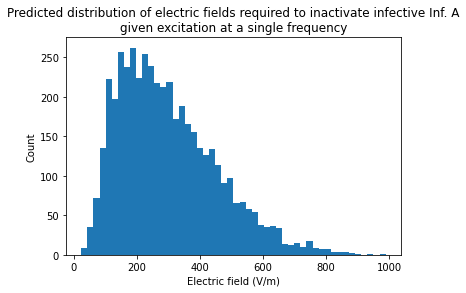
\includegraphics[width=\textwidth]{biology/output_35_1.png}
\end{figure}



microwave diathermy and hyperthermia; 

In female patients, much of the lung is shielded by breast tissues. However, since fat is not particularly conductive, 

The spike proteins, essential to the virus's infectivity, are 


Several more recent papers \cite{Theoretical2020} on the technique have been published, but these are largely pseudoscientific and lack detail. 

We are not aware of any clinical trial using microwave at these frequencies.

\cite{neuroinvasive2020}

On the other hand, increasing evidence
shows that CoVs may first invade peripheral nerve terminals, and
then gain access to the CNS via a synapse‐connected route.

to, er, head them off at the head.

alveolar damage

https://www.nature.com/articles/s41379-020-0595-z

Inclusion criteria:

preliminary

dyspnea

Patients where disease progression indicates that hypoxic respiratory failure is likely to occur.

Dyspnea
Oxygen saturation
CT: lung opacities

Without metal piercings or 




Non-thermal nerve stimulation leading to temporary paralysis has been reported. 

Since the reproductive organs are not involved in the infection; and they will not receive a dose above background.\cite{Organ2004}.





\citationneeded



(2) The application must contain sufficient information and material to enable the Minister to determine whether to issue the authorization and must include the following:

the name and contact information of the applicant 
the name and class of the device;
a description of the device and of the materials used in its manufacture and packaging;
a description of the features of the device that permit it to be used for the medical conditions, purposes and uses for which it is manufactured, sold or represented, including its performance specifications if those specifications are necessary for proper use;
the identifier of the device, including the identifier of any medical device that is part of a system, test kit, medical device group, medical device family or medical device group family;
the name and contact information of the manufacturer as they appear on the device label;
the address where the device is manufactured, if the address is different from the one provided in the contact information under paragraph (f);
the diagnosis, treatment, mitigation or prevention for which the device is required;
a list of the countries other than Canada where the device has been sold, the total number of units sold in those countries and a summary of any reported problems with the device and of any recalls of the device in those countries;
the known information in relation to the quality, safety and effectiveness of the device;
the directions for use, unless directions are not required for the device to be used safely and effectively;
an attestation by the applicant that documented procedures are in place in respect of distribution records, complaint handling, incident reporting and recalls;
a copy of the label of the device;
the name of the qualified investigator and their qualifications, including their training and experience;
the name and contact information of the institution at which the clinical trial is proposed to be conducted;
the protocol of the proposed clinical trial, including the number of clinical trial subjects, the number of units of the device proposed to be used for the clinical trial, the hypothesis for and objective of the clinical trial, the period of time during which the clinical trial will be conducted and a copy of the informed consent form;
a written undertaking from the qualified investigator to:
conduct the clinical trial in accordance with the protocol provided by the applicant,
inform each clinical trial subject of any risks and benefits associated with the use of the device and obtain the subject's informed consent for its use, and
not permit the device to be used by any other person except under the direction of the qualified investigator; and
in the case of a Class III or IV device, for each clinical trial site, the name and contact information of the research ethics board that approved the protocol and informed consent form referred to in paragraph (p), if known at the time of submitting the application.
Class II devices
(3) Despite subsection (2), if the application for the authorization is in respect of a Class II COVID-19 medical device, the information and material set out in paragraphs (2)‍(c), (h) to (j), (n) and (q) may be omitted from the application.







Research question: 
Does 
Null Hypothesis: There is no difference in fluoride release between the Compomer and Glass- ionomer cement.
Alternate Hypothesis: There is a difference in fluoride release between the Compomer and Glass-ionomer cement.
Disease progression

Proposed intervention:



\section{Potential Benefits and Risks to Patients:}

\section{Operational Planning and Budgeting:}



Keysight / Agilent 83732B



\end{document}